\chapter{光子统计与相干函数}
\label{chap:04}

\begin{chapteropening}
前几章已经把光看成一串带标签的探测事件。现在要问的不是“平均有多亮”，而是“这些事件之间有没有关系”。如果两个时间门、两个探测器、两个频率通道或两个偏振通道里的光子只是各自随机到来，那么任何符合计数都只是偶然重合。如果它们比随机情形更常一起出现，或更少一起出现，事件表里就留下了光场统计的痕迹。Hanbury Brown--Twiss 实验、Glauber 相干理论和 Mandel 光子计数理论共同建立的，正是这套把事件表翻译成相干函数的语言 \citep{1956Natur.177...27B,1957RSPSA.242..300B,1958RSPSA.248..222B,1961AmJPh..29..539F,1963PhRv..130.2529G,1963PhRv..131.2766G,1965RvMP...37..231M,1995ocqo.book.....M,2000stop.book.....G,2007itcp.book.....W}。
\end{chapteropening}

\section{为什么先数事件对}

望远镜最后给出的不是一个抽象的“光场”，而是一张事件表。对第 \(j\) 个探测通道，可以写成
\[
  \mathcal{D}_j=\{t_{j,q},\nu_{j,q},p_{j,q},w_{j,q}\}_{q=1}^{N_j}.
\]
这里 \(t_{j,q}\) 是第 \(q\) 个事件的到达时间，通常用秒表示；\(\nu_{j,q}\) 是它落入的频率或波段；\(p_{j,q}\) 是偏振、探测器或电子通道标签；\(w_{j,q}\) 是质量权重，例如背景概率、坏像素掩膜或死时间修正。光学 HBT 与强度干涉常要处理 ns 量级的电子响应；X 射线和伽马射线事件表可能有 \(\mu{\rm s}\) 到 ms 的时间戳；普通成像和低时间分辨光谱若只保存积分后的像素强度，就已经把许多光子之间的时间关系平均掉了。

把连续时间切成宽度为 \(\Delta t\) 的小门，第 \(k\) 个时间门中的计数为
\begin{equation}
  N_{j,k}(\Delta t)=\sum_q w_{j,q}\,
  \mathbf{1}\!\left(t_k\leq t_{j,q}<t_k+\Delta t\right),
  \qquad
  \widehat r_{j,k}=\frac{N_{j,k}}{\Delta t}.
  \label{eq:ch04-count-bin}
\end{equation}
\begin{formulaexplain}
\(N_{j,k}\) 是通道 \(j\) 在第 \(k\) 个时间门内的计数；\(w_{j,q}\) 是事件权重；\(\mathbf 1(\cdots)\) 选择落入门内的事件；\(\widehat r_{j,k}\) 是该门的估计计数率。它把事件表变成可相关的时间序列。
\end{formulaexplain}
\(N_{j,k}\) 是无量纲计数，\(\widehat r_{j,k}\) 的单位是 \({\rm s^{-1}}\)。如果 \(\Delta t=1\,{\rm ns}\)，平均光子率为 \(10^6\,{\rm s^{-1}}\)，那么一个时间门内的平均计数只有 \(10^{-3}\)。也就是说，绝大多数 bin 是 0，少数 bin 是 1，同一个 bin 里有两个光子的概率很小。强度相关因此不是从一条肉眼可见的“光变曲线起伏”读出来的，而是从 \(10^8\) 到 \(10^{12}\) 个时间门或事件对的微小 excess 里累加出来的。

这立刻解释了为什么二阶计数理论里出现的是阶乘矩，而不是普通二阶矩：
\begin{equation}
  \left\langle N(N-1)\right\rangle.
  \label{eq:ch04-factorial-moment}
\end{equation}
\begin{formulaexplain}
\(N\) 是一个时间门内的光子数；\(N(N-1)\) 是不同光子组成的有序事件对数；尖括号表示统计平均。它比 \(N^2\) 少掉同一个光子和自己配对的假项。
\end{formulaexplain}
若一个时间门里有 \(N\) 个光子，可以组成 \(N^2\) 个“带顺序的选择”，但其中有 \(N\) 个是同一个光子和自己配对。符合探测不允许这样的自配对。一个 START 脉冲和一个 STOP 脉冲必须来自两个探测事件，因此可用的有序光子对数是 \(N(N-1)\)。这就是正规序算符在光电探测理论中的物理含义：探测器数的是不同的吸收事件，不是同一个事件的平方。Glauber 的相干函数把这一点写进算符次序，Mandel 的计数理论把它写进计数分布 \citep{1963PhRv..130.2529G,1963PhRv..131.2766G,1965RvMP...37..231M}。

\begin{figure}[tbp]
\centering
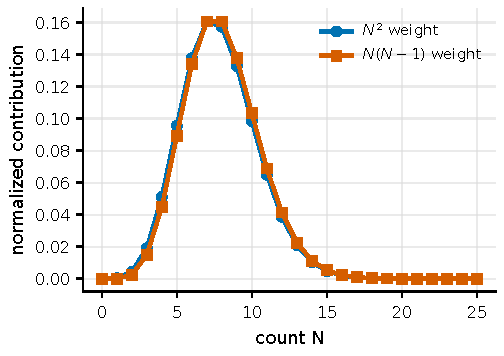
\includegraphics[width=0.86\linewidth]{figures/generated/chapter_04/ch04_factorial_moments.pdf}
\caption{Poisson 计数分布中，普通二阶矩 \(N^2\) 和阶乘矩 \(N(N-1)\) 对不同 \(N\) 的权重不同。符合探测只关心不同光子组成的光子对，因此 \(N(N-1)\) 自动去掉了同一光子的自配对项。}
\label{fig:ch04-factorial-moments}
\end{figure}

事件对还必须和仪器效应分开。单光子探测器在一次触发后通常有一段不能再次响应的死时间。APD、PMT 或 SiPM 的死时间可以是 \(10\)--\(100\,{\rm ns}\)，而可见光热光的相干时间常在 ps 或更短。若直接在同一个探测器上做自相关，零延迟附近会被死时间挖出一个仪器空洞；afterpulsing 又可能在非零延迟制造假峰。因此许多零延迟光子统计实验会先用分束器把同一束光分到两个独立探测器，再做交叉相关。Guerin 等人的恒星热光聚束实验就是这种结构：1 m 望远镜、多模光纤、分束器、两只 APD 和 TDC 延迟直方图。他们的 APD 死时间约 \(22\,{\rm ns}\)，而光学相干时间只有 ps 量级；若不分束，天体的聚束峰会和探测器恢复时间纠缠在一起 \citep{2017MNRAS.472.4126G}。

\begin{figure}[tbp]
\centering
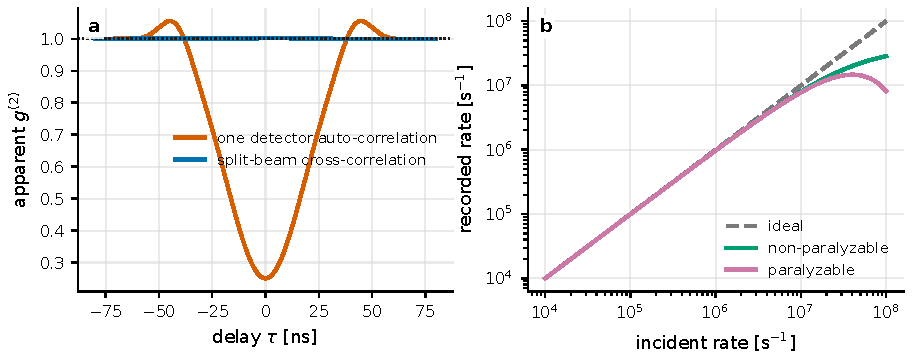
\includegraphics[width=0.92\linewidth]{figures/generated/chapter_04/ch04_deadtime_pileup_bias.pdf}
\caption{死时间、pile-up 和 afterpulsing 对短延迟相关的影响。左图显示单探测器自相关会出现零延迟空洞和非零延迟假峰，分束后的双探测器交叉相关更接近真实热光聚束峰；右图显示入射光子率升高后，不同死时间模型会给出不同的记录率饱和曲线。}
\label{fig:ch04-deadtime-pileup}
\end{figure}

\begin{longtable}{p{0.20\linewidth}p{0.25\linewidth}p{0.42\linewidth}}
\toprule
量 & 单位和典型范围 & 物理意义 \\
\midrule
\(t_{j,q}\) & s；精度从 ns 到 ms & 单个探测事件的到达时间；相关函数的横轴由事件时间差构成。 \\
\(\Delta t\) & ps 到 s & 人为选择的计数门宽或电子采样间隔；若远大于相干时间，会稀释聚束峰。 \\
\(r_j\) & \({\rm s^{-1}}\)；光学 HBT 常 \(10^5\)--\(10^7\) & 第 \(j\) 个通道的平均计数率，决定 shot noise 和可用事件对数。 \\
\(\tau_d\) & ns 到 \(\mu{\rm s}\) & 探测器死时间；若和待测延迟相近，需要用分束、交叉相关或死时间模型修正。 \\
\(H_{AB}(\tau)\) & 每个延迟 bin 的计数 & 两通道事件对的延迟直方图；归一化后给出 \(g^{(2)}\)。 \\
\bottomrule
\end{longtable}

\section{一阶和二阶相干到底在问什么}

相干函数看起来像形式化定义，但每一阶都对应一个很朴素的问题。一阶相干问：“同一束光在两个时刻的电场振幅和相位是否还相互记得？”二阶相干问：“两个强度探测事件是否比随机情形更容易成对出现？”前一个问题属于电场相位记忆，后一个问题属于光子到达的联合概率。振幅干涉主要利用前者，强度干涉和 HBT 主要利用后者。

在探测面上，把正频率电场算符写作 \(\hat E^{(+)}(t)\)，负频率部分写作 \(\hat E^{(-)}(t)\)。一阶相干函数定义为
\begin{equation}
  G^{(1)}(t_1,t_2)
  =
  \left\langle
    \hat E^{(-)}(t_1)\hat E^{(+)}(t_2)
  \right\rangle,
  \qquad
  g^{(1)}(\tau)=\frac{G^{(1)}(t,t+\tau)}{G^{(1)}(t,t)} .
  \label{eq:ch04-g1}
\end{equation}
\begin{formulaexplain}
\(G^{(1)}\) 是一阶场相关函数；\(\hat E^{(+)}\)、\(\hat E^{(-)}\) 是正、负频率场算符；\(g^{(1)}\) 是归一化结果；\(\tau\) 是时间延迟。它测的是电场相位和振幅隔一段时间后还保留多少记忆。
\end{formulaexplain}
\(G^{(1)}\) 带有强度单位，归一化后的 \(g^{(1)}\) 无量纲。若光场平稳，相关只依赖延迟 \(\tau=t_2-t_1\)。当 \(|g^{(1)}(\tau)|\) 接近 1 时，延迟 \(\tau\) 后的电场仍能和原来的电场形成清晰干涉；当它接近 0 时，相位已经基本失去记忆。振幅干涉仪测到的条纹可见度，正是空间版本的 \(g^{(1)}\)。

光谱带宽决定了这种相位记忆能维持多久。若滤光片中心波长为 \(\lambda\)，带宽为 \(\Delta\lambda\ll\lambda\)，频率带宽近似为
\begin{equation}
  \Delta\nu \simeq \frac{c\,\Delta\lambda}{\lambda^2},
  \qquad
  \tau_c \sim \frac{1}{\Delta\nu}
  \simeq \frac{\lambda^2}{c\,\Delta\lambda}.
  \label{eq:ch04-coherence-time}
\end{equation}
\begin{formulaexplain}
\(\Delta\nu\) 是频率带宽；\(\Delta\lambda\) 是波长带宽；\(\lambda\) 是中心波长；\(c\) 是光速；\(\tau_c\) 是相干时间。这个式子把滤光片带宽直接换成热光相关峰的时间尺度。
\end{formulaexplain}
\(\tau_c\) 是相干时间，单位是秒。它不是探测器时间分辨率，而是光本身由带宽决定的相位记忆时间。例如 \(\lambda=780\,{\rm nm}\)、\(\Delta\lambda=1\,{\rm nm}\) 时，\(\tau_c\) 约为 \(2\,{\rm ps}\)。普通可见光宽带滤光片给出的热光相干时间通常远短于 ns 电子响应。这个数量级会在恒星聚束实验、窄线 photon-correlation spectroscopy 和第 \ref{chap:05} 章的空间强度干涉中反复出现 \citep{2008AIPC..984..216D,2009A&A...507.1719F,2017MNRAS.472.4126G}。

\Needspace{13\baselineskip}
二阶相干函数把问题从“电场是否还记得相位”改成“两个探测事件是否相关”。量子探测理论给出的定义是
\begin{equation}
  G^{(2)}(t_1,t_2)
  =
  \left\langle
    \hat E^{(-)}(t_1)\hat E^{(-)}(t_2)
    \hat E^{(+)}(t_2)\hat E^{(+)}(t_1)
  \right\rangle,
  \qquad
  g^{(2)}(\tau)=
  \frac{G^{(2)}(t,t+\tau)}
  {G^{(1)}(t,t)\,G^{(1)}(t+\tau,t+\tau)} .
  \label{eq:ch04-g2}
\end{equation}
\begin{formulaexplain}
\(G^{(2)}\) 是二阶正规序场相关；分子数共同探测，分母给随机符合基线；\(g^{(2)}\) 是归一化结果。它测的是光子是否倾向于成对到达。
\end{formulaexplain}
这个式子可以逐项读。右端分母是两个时刻各自的平均强度，代表“若两个探测完全独立，随机符合数应该是多少”。分子是两个探测事件共同发生的强度相关。归一化以后，\(g^{(2)}\) 无量纲。独立 Poisson 到达给 \(g^{(2)}=1\)；若 \(g^{(2)}(0)>1\)，零延迟附近的光子对比随机情形更多，称为聚束；理想单一时空偏振模式的热光给 \(g^{(2)}(0)=2\)。若 \(g^{(2)}(0)<1\)，零延迟符合被压低，称为反聚束；这不能由正定经典强度涨落解释，是单光子源和共振荧光的标准量子光学判据 \citep{1977PhRvL..39..691K,1979OptL....4..205M,1986PhRvA..33.4033Y,1993PhRvL..71.4287Z,2005Natur.436...87B}。

在工程估算中，人们常把同一个定义写成连续强度形式
\begin{equation}
  g^{(2)}(\tau)=
  \frac{\left\langle I(t)I(t+\tau)\right\rangle}
       {\left\langle I(t)\right\rangle^2}
  \label{eq:ch04-classical-g2}
\end{equation}
\begin{formulaexplain}
\(I(t)\) 是强度或探测电流；\(\tau\) 是延迟；分子是强度共同涨落；分母是平均强度平方。这个经典写法适合工程估算，但必须说明 \(I(t)\) 是否已被探测器响应卷积。
\end{formulaexplain}
但这行式子要谨慎使用。这里的 \(I(t)\) 可以是理想瞬时强度，也可以是探测器输出电流、TDC 事件率或采样后的 ADC 值。若 \(I(t)\) 已经被 \(4\,{\rm ns}\) 电子响应卷积，式中得到的是响应后的 \(g^{(2)}\)，不是光场本身 ps 宽度的相关峰。许多天文强度相关信号并不是“没有聚束”，而是聚束峰被有限时间响应、多个模式和背景光压低到 \(10^{-3}\)、\(10^{-6}\) 甚至更小。

\section{计数分布怎样进入相关估计}

单模成对因子 \(b_2\) 在事件表中表现为固定时间门计数的阶乘矩。只看平均光子率不够，因为不同光场可以有相同的平均亮度，却有完全不同的计数起伏。把一个固定时间门里的计数记为 \(N\)，均值为 \(\bar{N}\)，方差为 \(\sigma_N^2\)。Mandel 参数定义为
\begin{equation}
  Q=\frac{\sigma_N^2-\bar{N}}{\bar{N}}.
  \label{eq:ch04-mandel-q}
\end{equation}
\begin{formulaexplain}
\(Q\) 是 Mandel 参数；\(\sigma_N^2\) 是时间门计数方差；\(\bar N\) 是平均计数。它用 Poisson 方差 \(\sigma_N^2=\bar N\) 作零点，区分超 Poisson、Poisson 和亚 Poisson 统计。
\end{formulaexplain}
这个定义把 Poisson shot noise 当作零点。\(Q=0\) 表示方差正好等于均值；\(Q>0\) 表示超 Poisson 起伏，常见于热光或强度涨落很大的混沌光；\(Q<0\) 表示亚 Poisson 起伏，意味着计数比 Poisson 更规整，是非经典统计的重要信号。

\(Q\) 和零延迟二阶相干的联系来自一个简单代数恒等式：
\[
  \left\langle N(N-1)\right\rangle
  =
  \left\langle N^2\right\rangle-\bar{N}
  =
  \sigma_N^2+\bar{N}^2-\bar{N}.
\]
因此
\begin{equation}
  g^{(2)}(0)=
  \frac{\left\langle N(N-1)\right\rangle}{\bar{N}^2}
  =
  1+\frac{Q}{\bar{N}}.
  \label{eq:ch04-q-g2}
\end{equation}
\begin{formulaexplain}
\(g^{(2)}(0)\) 是零延迟二阶相干；\(\langle N(N-1)\rangle\) 是阶乘矩；\(\bar N\) 是平均门计数；\(Q\) 是 Mandel 参数。它把计数方差语言和光子成对到达语言连起来。
\end{formulaexplain}
这里的 \(N\) 是一个时间门内的计数，不是整晚观测的总计数。若把时间门加宽，\(\bar{N}\) 增大，许多彼此不相干的时间模式会被平均进同一个 \(N\)，于是同一内禀光场的 \(g^{(2)}(0)-1\) 会被稀释。这个式子也是一个提醒：不能只报 \(Q\) 或只报 \(g^{(2)}(0)\)，还要说明时间门宽、模式数和平均计数。

\begin{figure}[tbp]
\centering
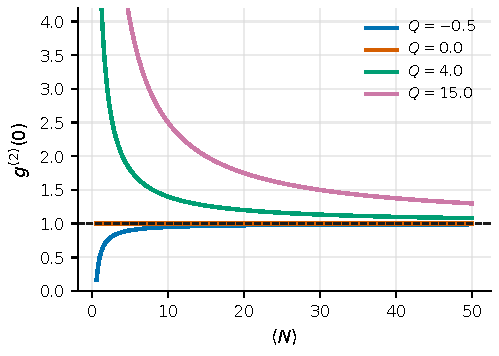
\includegraphics[width=0.86\linewidth]{figures/generated/chapter_04/ch04_mandel_q_g2.pdf}
\caption{在固定时间门内，Mandel \(Q\) 通过 \(g^{(2)}(0)=1+Q/\langle N\rangle\) 改变零延迟二阶相干。低平均计数时，同样的 \(Q\) 会造成更大的 \(g^{(2)}(0)\) 偏离；平均许多模式后，曲线逐渐回到 1。}
\label{fig:ch04-mandel-q-g2}
\end{figure}

\Needspace{10\baselineskip}
单模热态在时间门计数语言中写成 Bose--Einstein 分布：
\begin{equation}
  P(N)=\frac{\bar{N}^{\,N}}{(1+\bar{N})^{N+1}},
  \qquad
  \sigma_N^2=\bar{N}+\bar{N}^2,
  \qquad
  g^{(2)}(0)=2.
  \label{eq:ch04-thermal-count}
\end{equation}
\begin{formulaexplain}
\(P(N)\) 是单模热光计数概率；\(\bar N\) 是该时间门内的平均计数；\(\sigma_N^2\) 是方差；\(g^{(2)}(0)=2\) 是理想聚束峰。它把热态光子数统计改写成可用于事件表的形式。
\end{formulaexplain}
方差里的 \(\bar{N}\) 是 shot noise，\(\bar{N}^2\) 是热光的波动噪声。物理图像是这样的：热光的电场由许多随机相位的微小贡献叠加，瞬时强度会形成随机明暗起伏；探测器在亮斑时更容易接连记录多个光子，于是零延迟附近的符合计数升高。这就是 HBT 聚束。

真实望远镜通常不会只收一个单一模式。若 \(M\) 个强度相近且相互独立的热光模式被同一个探测器平均，方差和聚束峰变成
\begin{equation}
  \sigma_N^2=\bar{N}+\frac{\bar{N}^2}{M},
  \qquad
  g^{(2)}(0)=1+\frac{1}{M}.
  \label{eq:ch04-multimode}
\end{equation}
\begin{formulaexplain}
\(M\) 是独立热光模式数；\(\bar N^2/M\) 是被多模平均后的额外波动噪声；\(g^{(2)}(0)-1=1/M\) 是聚束 excess。它解释了为什么天文多模数据里的峰高远小于 1。
\end{formulaexplain}
这里的 \(M\) 可以来自两个偏振、多个空间 speckle、宽光谱里的多个频率模式，也可以来自一个时间门内包含的多个相干时间。未分偏振的热光点源通常已经有 \(M_{\rm pol}\simeq2\)，理想峰高从 2 降到 1.5。若电子时间门比相干时间宽 \(10^3\) 倍，时间模式平均又会把 excess 再压低约 \(10^3\) 倍。这就是为什么天文 HBT 图上常看到的是 \(g^{(2)}-1\) 的小数，而不是教科书里的 1。

相干态在同样的时间门里给 Poisson 计数：
\begin{equation}
  P(N)=e^{-\bar{N}}\frac{\bar{N}^N}{N!},
  \qquad
  \sigma_N^2=\bar{N},
  \qquad
  g^{(2)}(\tau)=1.
  \label{eq:ch04-poisson-count}
\end{equation}
\begin{formulaexplain}
\(P(N)\) 是 Poisson 分布；\(\bar N\) 是平均计数；\(N!\) 归一化离散计数；\(\sigma_N^2=\bar N\) 是 shot noise；\(g^{(2)}=1\) 表示没有过量或不足的事件对。它是相干态在事件时间门中的写法。
\end{formulaexplain}
理想激光可以有很长的一阶相干时间，却没有热光式二阶聚束。因此“相干”一词在天文学里要分清含义：射电 maser、脉冲星相干曲率辐射、天体激光候选线和非热同步辐射，可能在一阶相干、二阶相干和多源平均上表现出不同统计。许多天体 maser 是大量小 coherence cell 的叠加，观测到的 \(g^{(2)}\) 不一定像实验室单模激光 \citep{1977ApJ...212..800C,1991ApJ...383..808M,2004A&A...428..497J,2005MNRAS.364..731J,2005NewA...10..361J,2008AIPC..984..216D,2009A&A...507.1719F}。

\section{Siegert 关系把 HBT 和场相干联系起来}

现在可以回到 HBT 的核心问题：为什么强度相关能告诉我们场相干信息？关键是热光或更一般的高斯混沌光有一个特殊性质。电场是许多独立小贡献的随机叠加时，复电场近似服从高斯统计；四阶矩可以拆成二阶矩的组合。用经典符号写，直观上就是
\[
  \left\langle I(t)I(t+\tau)\right\rangle
  =
  \left\langle I\right\rangle^2
  +
  \left|G^{(1)}(\tau)\right|^2
\]
再除以平均强度平方，就得到 Siegert 关系：
\begin{equation}
  g^{(2)}(\tau)=1+\zeta\left|g^{(1)}(\tau)\right|^2 .
  \label{eq:ch04-siegert}
\end{equation}
\begin{formulaexplain}
\(g^{(2)}-1\) 是强度相关 excess；\(g^{(1)}\) 是归一化一阶场相干；\(\zeta\) 是模式、偏振、背景和响应造成的可见度因子。它是 HBT 从强度相关读出场相干模平方的核心桥梁。
\end{formulaexplain}
\(\zeta\) 是可见度因子，满足 \(0<\zeta\leq1\)。理想单一时空偏振模式有 \(\zeta=1\)；未分偏振、多空间模式、有限带宽平均、背景光和仪器响应都会降低 \(\zeta\)。如果源光子只占两个通道总计数的比例分别为 \(f_A\) 和 \(f_B\)，且背景不相关也没有自己的聚束峰，那么相关峰幅度还要近似乘上 \(f_A f_B\)。

\begin{figure}[tbp]
\centering
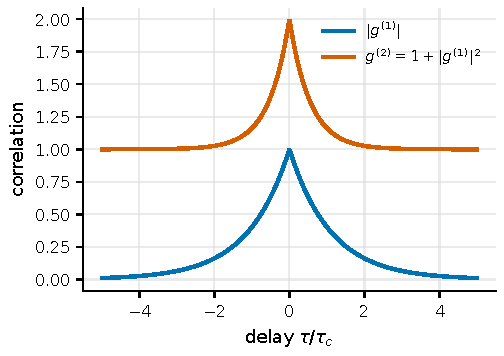
\includegraphics[width=0.86\linewidth]{figures/generated/chapter_04/ch04_siegert_relation.pdf}
\caption{热光的 Siegert 关系把一阶场相干的衰减转化为二阶强度聚束峰。若 \(|g^{(1)}|\) 随延迟以相干时间 \(\tau_c\) 衰减，\(g^{(2)}-1\) 以 \(|g^{(1)}|^2\) 衰减，并在大延迟回到无相关值 0。实际峰高还要乘以模式数、背景和时间响应因子。}
\label{fig:ch04-siegert}
\end{figure}

式 \eqref{eq:ch04-siegert} 的意义很大。左边是事件表可测的强度相关；右边的 \(g^{(1)}\) 是电场相干，可由光谱的傅里叶变换得到，也可由振幅干涉仪的可见度测得。若光谱近似矩形，\(|g^{(1)}(\tau)|^2\) 近似 \({\rm sinc}^2(\Delta\nu\tau)\)；若谱线近似 Lorentzian，\(|g^{(1)}|\) 是指数衰减；若谱线近似 Gaussian，\(|g^{(1)}|^2\) 也是 Gaussian。窄谱线 photon-correlation spectroscopy 正是利用 \(g^{(2)}(\tau)\) 的宽度反推谱线宽度。对于 \(\eta\) Carinae 附近的 Fe II 或 O I 天体激光候选线，普通光谱仪很难达到 \(R\sim10^8\) 的分辨率，而 ns 量级的强度相关可以对 MHz 到 GHz 线宽给出独立约束 \citep{2005NewA...10..361J,2008AIPC..984..216D,2014ApJ...789L..10T}。

Siegert 关系也是第 \ref{chap:05} 章空间强度干涉的入口。把时间延迟 \(\tau\) 换成两台望远镜之间的空间基线 \(\mathbf{B}\)，\(g^{(1)}\) 就变成天空亮度分布的复可见度，强度相关测到的 excess 与 \(|g^{(1)}|^2\) 成正比。也就是说，HBT 不需要把两台望远镜的电场直接合束，却仍能通过强度涨落的同步程度得到可见度模平方。这一结论成立的前提，就是源光近似热光或高斯混沌光，并且仪器归一化没有把背景、模式数和时间响应混在一起。

这些前提不能省略。理想相干态满足长程 \(g^{(1)}\)，但 \(g^{(2)}=1\)，因此不服从热光式 \(1+|g^{(1)}|^2\)。反聚束光、压缩光、单光子源、强烈非平稳脉冲和少数相干子源叠加都可能打破式 \eqref{eq:ch04-siegert}。实验室量子光学已经在许多体系里测到非经典 \(g^{(2)}\)；天文上更常见的情况是混合场，例如许多非热小源平均后近似热光，或热连续谱上叠加窄非热线 \citep{1965PhRv..140..676T,1977PhRvL..39..691K,1979OptL....4..205M,2000PhRvA..62d3816S,2008PhRvA..78f1802S,2012PhRvL.109n7404Z,2020MNRAS.491.5789L}。

\section{从理想相关到望远镜里的估计量}

真实探测器测到的不是无限窄时间响应下的 \(g_{\rm true}^{(2)}\)，而是它和仪器响应的卷积：
\begin{equation}
  g_{\rm obs}^{(2)}(\tau)-1 =
  \int_{-\infty}^{+\infty}
  \left[g_{\rm true}^{(2)}(\tau')-1\right]
  R_{\Delta t}(\tau-\tau')\,d\tau',
  \label{eq:ch04-response-convolution}
\end{equation}
\begin{formulaexplain}
\(g_{\rm true}^{(2)}\) 是光场本征相关；\(g_{\rm obs}^{(2)}\) 是观测相关；\(R_{\Delta t}\) 是归一化仪器响应函数；\(\tau'\) 是积分变量。这个卷积说明有限时间响应会拉宽并压低窄相关峰。
\end{formulaexplain}
其中 \(R_{\Delta t}\) 的面积归一化为 1，宽度由探测器 jitter、电子带宽、采样窗口和分析 bin 共同决定。这个式子说明了一个容易误解的事实：卷积主要守住相关峰的面积，却会把窄峰拉宽、压低。若内禀峰宽 \(\tau_c\) 远小于有效响应宽度 \(\Delta t_{\rm eff}\)，峰值近似按
\begin{equation}
  C_{\rm obs}\equiv g_{\rm obs}^{(2)}(0)-1
  \simeq
  C_{\rm true}\,
  \frac{\tau_c}{\Delta t_{\rm eff}}\,
  \frac{1}{M_{\rm pol}M_{\rm sp}}\,
  f_A f_B
  \label{eq:ch04-contrast-dilution}
\end{equation}
\begin{formulaexplain}
\(C_{\rm obs}\) 和 \(C_{\rm true}\) 是观测与理想峰高；\(\tau_c/\Delta t_{\rm eff}\) 是时间稀释；\(M_{\rm pol},M_{\rm sp}\) 是偏振和空间模式数；\(f_Af_B\) 是背景稀释。它是望远镜中相关峰幅度的误差预算式。
\end{formulaexplain}
被稀释。这里 \(C_{\rm true}\) 是理想峰高；\(M_{\rm pol}\) 和 \(M_{\rm sp}\) 是偏振和空间模式数；\(f_A,f_B\) 是两通道里源光子占总计数的比例。式 \eqref{eq:ch04-contrast-dilution} 是数量级公式。精确分析应把实测响应函数、光谱给出的 \(|g^{(1)}|^2\)、背景和电子学相关一起放进模型。

\begin{figure}[tbp]
\centering
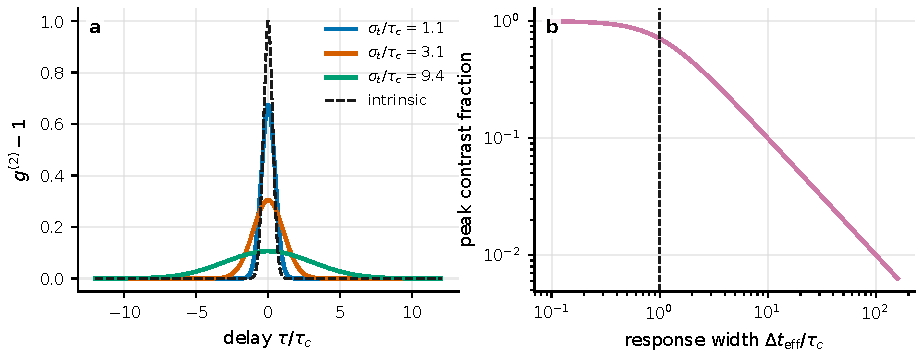
\includegraphics[width=0.95\linewidth]{figures/generated/chapter_04/ch04_response_convolution.pdf}
\caption{有限时间响应会把窄的热光聚束峰拉宽并压低。左图中虚线是内禀 ps 量级峰，实线是不同响应宽度卷积后的观测峰；右图显示当 \(\Delta t_{\rm eff}\gg\tau_c\) 时，零延迟峰高近似按 \(\tau_c/\Delta t_{\rm eff}\) 下降。}
\label{fig:ch04-response-convolution}
\end{figure}

Guerin 等人的恒星聚束实验给出了一组有用的标尺。中心波长约 \(7800\,\text{\AA}\)，最窄滤光片宽度 \(10\,\text{\AA}\)，对应 \(\Delta\nu\simeq5\times10^{11}\,{\rm Hz}\) 和 \(\tau_c\simeq1.6\)--\(2\,{\rm ps}\)。APD 的单光子时间 jitter 约 \(500\,{\rm ps}\)，两个探测器的相对响应峰宽约 \(700\,{\rm ps}\)。理想热光 \(C_{\rm true}=1\)，但卷积后预期观测峰只有 \(C_{\rm obs}\simeq2.2\times10^{-3}\)；实验室热源测到 \((2.01\pm0.09)\times10^{-3}\)，三颗亮星也给出约 \(1.8\)--\(2.0\times10^{-3}\) 的峰 \citep{2017MNRAS.472.4126G}。因此望远镜相关图上直接出现的通常不是 \(g^{(2)}(0)=2\)，而是 \(1+10^{-3}\)、\(1+10^{-6}\) 或更小的 excess。

事件表里的交叉相关估计量可以写成延迟直方图。对两个通道 \(A,B\)，bin 宽为 \(\delta\tau\)，总 live time 为 \(T\)，
\begin{equation}
  H_{AB}(\tau_m)
  =
  \sum_{i\in A}\sum_{j\in B}
  \mathbf{1}\!\left(
    \tau_m-\frac{\delta\tau}{2}
    \leq t_{B,j}-t_{A,i}
    < \tau_m+\frac{\delta\tau}{2}
  \right),
  \label{eq:ch04-delay-histogram}
\end{equation}
\begin{formulaexplain}
\(H_{AB}(\tau_m)\) 是通道 \(A,B\) 的事件对延迟直方图；\(t_{B,j}-t_{A,i}\) 是一对事件的延迟；\(\tau_m\) 是延迟 bin 中心；\(\delta\tau\) 是 bin 宽。它把事件表直接变成相关函数的原始计数。
\end{formulaexplain}
\begin{equation}
  \widehat g^{(2)}_{AB}(\tau_m)
  =
  \frac{H_{AB}(\tau_m)}
  {r_A r_B\,\delta\tau\,T}.
  \label{eq:ch04-g2-estimator}
\end{equation}
\begin{formulaexplain}
\(\widehat g^{(2)}_{AB}\) 是二阶相关估计量；\(r_A,r_B\) 是两通道平均计数率；\(\delta\tau T\) 给出延迟 bin 和 live time；分母是随机符合期望。它把直方图归一化到“无相关时等于 1”的尺度。
\end{formulaexplain}
\(H_{AB}\) 是观测到的事件对数；分母是同样 live time、同样 bin 宽、同样平均计数率下的随机符合期望，所以 \(\widehat g^{(2)}\) 无量纲。真实分析常不用解析分母，而用大时间偏移、不同观测段、偏振错配或 off-source 通道构造参考直方图 \(H_{\rm ref}(\tau)\)，再取比值或差值。这样可以吸收 TDC bin 宽不均、电子串扰、慢变透明度和采样窗口边缘效应。

\begin{figure}[tbp]
\centering
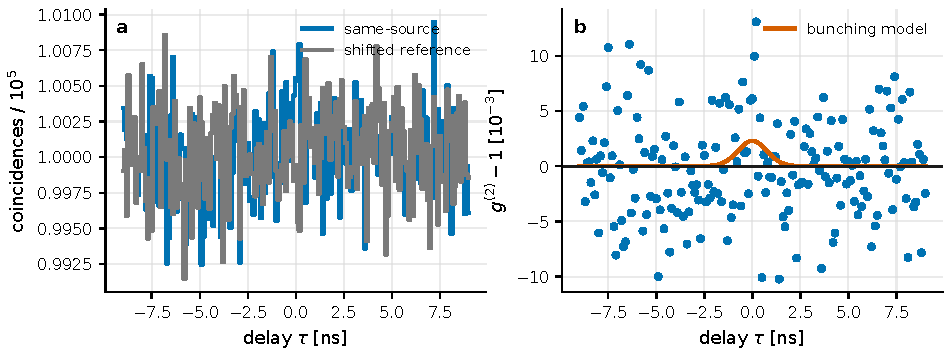
\includegraphics[width=0.95\linewidth]{figures/generated/chapter_04/ch04_delay_histogram_estimator.pdf}
\caption{延迟直方图估计量的结构。左图中同源事件对直方图在零延迟附近比移位参考直方图多出很小的符合数；右图把差值按随机符合数归一化后得到 \(g^{(2)}-1\)，峰值只有 \(10^{-3}\) 量级。真实观测还要加入死时间、背景和响应函数修正。}
\label{fig:ch04-delay-histogram}
\end{figure}

误差主要来自随机符合对数。若某个延迟 bin 中随机符合数为 \(N_{\rm pair}\)，shot-noise 误差的数量级是
\begin{equation}
  \sigma\!\left[\widehat g^{(2)}(\tau)\right]\sim N_{\rm pair}^{-1/2}.
  \label{eq:ch04-shot-noise}
\end{equation}
\begin{formulaexplain}
\(\sigma[\widehat g^{(2)}]\) 是相关估计量的统计误差；\(N_{\rm pair}\) 是该延迟 bin 中的随机符合对数。它说明强度相关的精度主要靠积累大量独立事件对。
\end{formulaexplain}
以两个 \(10^6\,{\rm s^{-1}}\) 通道、\(\delta\tau=100\,{\rm ps}\)、\(T=1\,{\rm hr}\) 为例，随机符合数约 \(3.6\times10^8\)，单 bin 统计误差约 \(5\times10^{-5}\)。如果聚束峰跨越多个 bin，可以拟合整个峰而不只看零延迟 bin；如果系统相关停在 \(10^{-3}\) 量级，继续增加曝光也不会替代 TDC、电子串扰和背景归一化修正。Guerin 等人的数据在修正 TDC spurious correlation 后接近 \(N^{-1/2}\) 标度；现代 VERITAS 和 MAGIC 系统则通过离线相关、GPU/FPGA 相关器和许多基线平均，把同一思想推广到空间强度干涉 \citep{2017MNRAS.472.4126G,2020NatAs...4.1164A,2024MNRAS.529.4387A}。

\Needspace{14\baselineskip}
二阶相关只用光子对。若同时保留三个望远镜或三个时间通道，可以定义三阶强度相关
\begin{equation}
  g^{(3)}_{123}=
  \frac{\left\langle I_1 I_2 I_3\right\rangle}
       {\left\langle I_1\right\rangle
        \left\langle I_2\right\rangle
        \left\langle I_3\right\rangle}.
  \label{eq:ch04-g3}
\end{equation}
\begin{formulaexplain}
\(g^{(3)}_{123}\) 是三通道归一化强度相关；\(I_1,I_2,I_3\) 是三个望远镜或时间通道的强度；分母给随机三重符合基线。它把统计对象从光子对推广到光子三元组。
\end{formulaexplain}
对于高斯混沌光，三阶相关包含三个二阶项和一个闭合三角形项：
\begin{equation}
  g^{(3)}_{123}
  =
  1
  +|\gamma_{12}|^2+|\gamma_{23}|^2+|\gamma_{31}|^2
  +2\,{\rm Re}\!\left(\gamma_{12}\gamma_{23}\gamma_{31}\right).
  \label{eq:ch04-g3-closure}
\end{equation}
\begin{formulaexplain}
\(\gamma_{ij}\) 是通道 \(i,j\) 的一阶相干度；模平方项来自三条基线；\({\rm Re}(\gamma_{12}\gamma_{23}\gamma_{31})\) 是闭合三角形项。它是三阶强度干涉恢复相位组合的入口。
\end{formulaexplain}
\(\gamma_{ij}\) 是第 \(i,j\) 个通道之间的一阶相干度。最后一项包含闭合相位，因此三阶强度相关原则上能把第 \ref{chap:05} 章中丢失的 Fourier 相位组合找回来。代价是噪声更大：光子三元组比光子对少得多，对系统误差也更敏感。Gamo 的早期理论、Ofir--Ribak 思路、Nuñez 等人的成像模拟和 CTA 相关研究都把高阶相关视作强度干涉成像的重要延伸 \citep{1966JOSA...56..441G,2012MNRAS.419..172N,2012MNRAS.424.1006N,2013APh....43..331D,2014SPIE.9146E..0ZD}。

\begin{figure}[tbp]
\centering
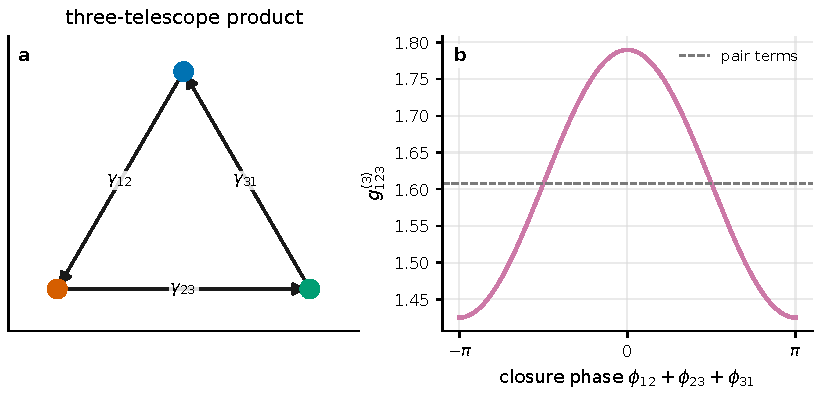
\includegraphics[width=0.92\linewidth]{figures/generated/chapter_04/ch04_g3_closure_phase.pdf}
\caption{三阶强度相关中闭合相位项的来源。左图中三台望远镜形成 \(\gamma_{12}\gamma_{23}\gamma_{31}\) 的闭合乘积；右图显示在固定 \(|\gamma_{ij}|\) 下，\(g^{(3)}\) 会随闭合相位余弦变化。二阶强度干涉只给 \(|\gamma|^2\)，三阶项才开始对相位组合敏感。}
\label{fig:ch04-g3-closure}
\end{figure}

频率分辨和偏振分辨的二阶相关写作
\begin{equation}
  g^{(2)}_{pq}(\nu_1,\nu_2,\tau)=
  \frac{
    \left\langle I_p(\nu_1,t)I_q(\nu_2,t+\tau)\right\rangle
  }{
    \left\langle I_p(\nu_1,t)\right\rangle
    \left\langle I_q(\nu_2,t)\right\rangle
  } .
  \label{eq:ch04-frequency-polarization-g2}
\end{equation}
\begin{formulaexplain}
\(p,q\) 是偏振通道；\(\nu_1,\nu_2\) 是两个频率通道；\(\tau\) 是时间延迟；分子是跨频率、跨偏振的强度共同涨落。它把二阶相关推广成可分析谱线、连续谱和偏振耦合的通道矩阵。
\end{formulaexplain}
\(p,q\) 是偏振通道，\(\nu_1,\nu_2\) 是频率或窄带滤光片中心。若两个频率采样同一条热谱线内的相干宽度，它们的强度涨落可以相关；若相隔远大于线宽，相关应回到 1。若两个偏振来自同一物理辐射过程，交叉偏振相关可能探测磁场几何或散射几何；若偏振通道混合了独立模式，聚束峰会被平均掉。对快速瞬变、脉冲星、FRB 光学对应体、天体 maser/laser 候选线和极端高时间分辨观测，保留事件级频率和偏振标签比只保存一条总光变曲线更有价值 \citep{2009A&A...507.1719F,2014ApJ...789L..10T,2024arXiv240418606N}。

\begin{figure}[tbp]
\centering
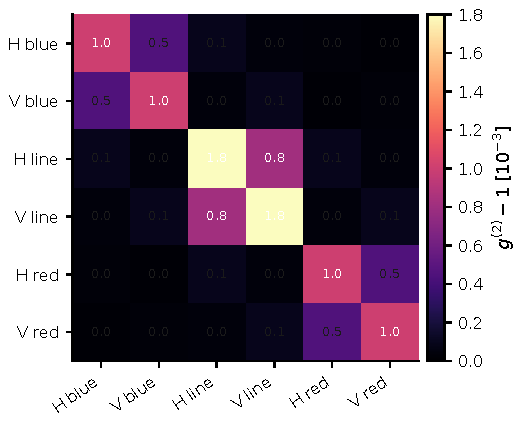
\includegraphics[width=0.72\linewidth]{figures/generated/chapter_04/ch04_frequency_polarization_matrix.pdf}
\caption{频率和偏振分辨 \(g^{(2)}\) 可以写成跨通道矩阵。谱线通道因为相干时间较长而有较高 excess，同一偏振通道的相关通常强于正交偏振通道；矩阵中的非对角元给出跨频率、跨偏振的共同涨落。}
\label{fig:ch04-frequency-polarization}
\end{figure}
